\documentclass[ignorenonframetext,]{beamer}
\setbeamertemplate{caption}[numbered]
\setbeamertemplate{caption label separator}{: }
\setbeamercolor{caption name}{fg=normal text.fg}
\beamertemplatenavigationsymbolsempty
\usepackage{lmodern}
\usepackage{amssymb,amsmath}
\usepackage{ifxetex,ifluatex}
\usepackage{fixltx2e} % provides \textsubscript
\ifnum 0\ifxetex 1\fi\ifluatex 1\fi=0 % if pdftex
  \usepackage[T1]{fontenc}
  \usepackage[utf8]{inputenc}
\else % if luatex or xelatex
  \ifxetex
    \usepackage{mathspec}
  \else
    \usepackage{fontspec}
  \fi
  \defaultfontfeatures{Ligatures=TeX,Scale=MatchLowercase}
\fi
% use upquote if available, for straight quotes in verbatim environments
\IfFileExists{upquote.sty}{\usepackage{upquote}}{}
% use microtype if available
\IfFileExists{microtype.sty}{%
\usepackage{microtype}
\UseMicrotypeSet[protrusion]{basicmath} % disable protrusion for tt fonts
}{}
\newif\ifbibliography
\hypersetup{
            pdfborder={0 0 0},
            breaklinks=true}
\usepackage{color}
\usepackage{fancyvrb}
\newcommand{\VerbBar}{|}
\newcommand{\VERB}{\Verb[commandchars=\\\{\}]}
\DefineVerbatimEnvironment{Highlighting}{Verbatim}{commandchars=\\\{\}}
% Add ',fontsize=\small' for more characters per line
\usepackage{framed}
\definecolor{shadecolor}{RGB}{248,248,248}
\newenvironment{Shaded}{\begin{snugshade}}{\end{snugshade}}
\newcommand{\KeywordTok}[1]{\textcolor[rgb]{0.13,0.29,0.53}{\textbf{{#1}}}}
\newcommand{\DataTypeTok}[1]{\textcolor[rgb]{0.13,0.29,0.53}{{#1}}}
\newcommand{\DecValTok}[1]{\textcolor[rgb]{0.00,0.00,0.81}{{#1}}}
\newcommand{\BaseNTok}[1]{\textcolor[rgb]{0.00,0.00,0.81}{{#1}}}
\newcommand{\FloatTok}[1]{\textcolor[rgb]{0.00,0.00,0.81}{{#1}}}
\newcommand{\ConstantTok}[1]{\textcolor[rgb]{0.00,0.00,0.00}{{#1}}}
\newcommand{\CharTok}[1]{\textcolor[rgb]{0.31,0.60,0.02}{{#1}}}
\newcommand{\SpecialCharTok}[1]{\textcolor[rgb]{0.00,0.00,0.00}{{#1}}}
\newcommand{\StringTok}[1]{\textcolor[rgb]{0.31,0.60,0.02}{{#1}}}
\newcommand{\VerbatimStringTok}[1]{\textcolor[rgb]{0.31,0.60,0.02}{{#1}}}
\newcommand{\SpecialStringTok}[1]{\textcolor[rgb]{0.31,0.60,0.02}{{#1}}}
\newcommand{\ImportTok}[1]{{#1}}
\newcommand{\CommentTok}[1]{\textcolor[rgb]{0.56,0.35,0.01}{\textit{{#1}}}}
\newcommand{\DocumentationTok}[1]{\textcolor[rgb]{0.56,0.35,0.01}{\textbf{\textit{{#1}}}}}
\newcommand{\AnnotationTok}[1]{\textcolor[rgb]{0.56,0.35,0.01}{\textbf{\textit{{#1}}}}}
\newcommand{\CommentVarTok}[1]{\textcolor[rgb]{0.56,0.35,0.01}{\textbf{\textit{{#1}}}}}
\newcommand{\OtherTok}[1]{\textcolor[rgb]{0.56,0.35,0.01}{{#1}}}
\newcommand{\FunctionTok}[1]{\textcolor[rgb]{0.00,0.00,0.00}{{#1}}}
\newcommand{\VariableTok}[1]{\textcolor[rgb]{0.00,0.00,0.00}{{#1}}}
\newcommand{\ControlFlowTok}[1]{\textcolor[rgb]{0.13,0.29,0.53}{\textbf{{#1}}}}
\newcommand{\OperatorTok}[1]{\textcolor[rgb]{0.81,0.36,0.00}{\textbf{{#1}}}}
\newcommand{\BuiltInTok}[1]{{#1}}
\newcommand{\ExtensionTok}[1]{{#1}}
\newcommand{\PreprocessorTok}[1]{\textcolor[rgb]{0.56,0.35,0.01}{\textit{{#1}}}}
\newcommand{\AttributeTok}[1]{\textcolor[rgb]{0.77,0.63,0.00}{{#1}}}
\newcommand{\RegionMarkerTok}[1]{{#1}}
\newcommand{\InformationTok}[1]{\textcolor[rgb]{0.56,0.35,0.01}{\textbf{\textit{{#1}}}}}
\newcommand{\WarningTok}[1]{\textcolor[rgb]{0.56,0.35,0.01}{\textbf{\textit{{#1}}}}}
\newcommand{\AlertTok}[1]{\textcolor[rgb]{0.94,0.16,0.16}{{#1}}}
\newcommand{\ErrorTok}[1]{\textcolor[rgb]{0.64,0.00,0.00}{\textbf{{#1}}}}
\newcommand{\NormalTok}[1]{{#1}}
\usepackage{longtable,booktabs}
\usepackage{caption}
% These lines are needed to make table captions work with longtable:
\makeatletter
\def\fnum@table{\tablename~\thetable}
\makeatother

% Prevent slide breaks in the middle of a paragraph:
\widowpenalties 1 10000
\raggedbottom

\AtBeginPart{
  \let\insertpartnumber\relax
  \let\partname\relax
  \frame{\partpage}
}
\AtBeginSection{
  \ifbibliography
  \else
    \let\insertsectionnumber\relax
    \let\sectionname\relax
    \frame{\sectionpage}
  \fi
}
\AtBeginSubsection{
  \let\insertsubsectionnumber\relax
  \let\subsectionname\relax
  \frame{\subsectionpage}
}

\setlength{\parindent}{0pt}
\setlength{\parskip}{6pt plus 2pt minus 1pt}
\setlength{\emergencystretch}{3em}  % prevent overfull lines
\providecommand{\tightlist}{%
  \setlength{\itemsep}{0pt}\setlength{\parskip}{0pt}}
\setcounter{secnumdepth}{0}
\usepackage[british]{babel}
\usepackage{graphicx,hyperref,anderson,url}
\usepackage{fontawesome}

\title[Assessing hurricane exposure for epidemiology]{Assessing exposure to hurricanes and other tropical
storms for epidemiological research}
\subtitle{NCAR Group Meeting Presentation}
\date{January 18, 2017}

\author[Brooke Anderson]{
  Brooke Anderson \\\medskip
  {\small \faEnvelope: \url{brooke.anderson@colostate.edu}} \\
  {\small \faGithub:  \url{www.github.com/geanders}}}

\institute[Colorado State University]{
  Department of Environmental \& Radiological Health Sciences \\
  Environmental Epidemiology Section \\
  Colorado State University}

\date{}

\begin{document}

\begin{frame}
  \titlepage
\end{frame}

\section{Motivation}\label{motivation}

\begin{frame}{Epidemiologic research on tropical storms}

\begin{block}{Outcomes studied for U.S. tropical storms}
\begin{itemize}
  \item Mortality 
  \begin{itemize}
    \item Direct deaths
    \item Indirect deaths
  \end{itemize}
  \item Cardiovascular events
  \item Birth rates
  \item Birth outcomes
\end{itemize}
\end{block}

\begin{block}{Focus of exposure assessment for this study}
Multi-storm studies with aggregated daily counts of outcomes (for example, daily deaths by county). 
\end{block}

\end{frame}

\begin{frame}{Assessing exposure}

\begin{block}{Challenge for epidemiological research}
How can we determine whether a county was exposed to a tropical storm?
\end{block}

Previous approaches have varied but include:

\begin{itemize}
\tightlist
\item
  Distance from storm track
\item
  Storm winds above a threshold
\item
  Evacuation orders
\item
  FEMA reports
\item
  Combined metric (property damage, power outages, gas shortages, etc.)
\end{itemize}

\end{frame}

\begin{frame}{Assessing exposure}

\begin{columns}
\begin{column}{0.7\textwidth}

\begin{center}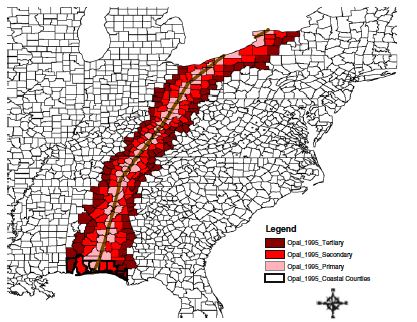
\includegraphics[width=\textwidth]{coastal_inland_mortality_figure} \end{center}
\vspace{-0.5cm}
\begin{center}
\footnotesize Czajkowski et al. 2011
\end{center}
\end{column}
\begin{column}{0.3\textwidth}
\small
\begin{block}{Example exposure assessment}
Czajkowski et al. (2011) classified counties based on distance to storm tracks to study mortality risks.
\end{block}
\end{column}
\end{columns}

\end{frame}

\begin{frame}{Assessing exposure}

\begin{columns}
\begin{column}{0.7\textwidth}

\begin{center}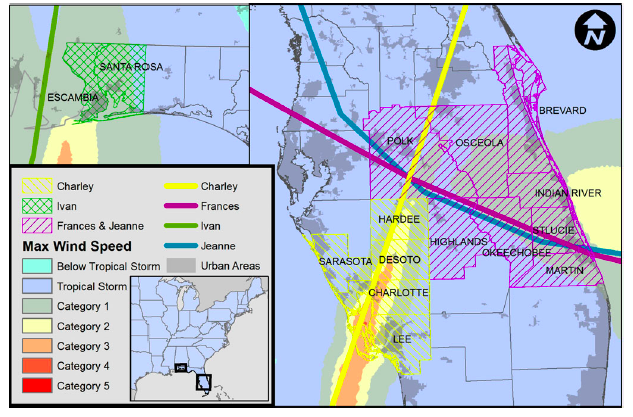
\includegraphics[width=\textwidth]{florida_direct_indirect_mortality_figure} \end{center}
\vspace{-0.6cm}
\begin{center}
\footnotesize McKinney et al. 2011
\end{center}
\end{column}
\begin{column}{0.3\textwidth}
\small
\begin{block}{Example exposure assessment}
McKinney et al. (2011) classified counties based on distance to storm tracks, evacuations, and wind to study mortality risk.
\end{block}
\end{column}
\end{columns}

\end{frame}

\begin{frame}{Project aims}

\begin{block}{Project aims}
\begin{itemize}
  \item Develop exposure classifications of all U.S. Atlantic basin tropical storms, 1988--2011, based on reasonable measurements of tropical storm hazards
  \item Assess agreement between hazard-based classifications for (1) storm severity and (2) county-specific classification
  \item Make exposure assessments accessible to other researchers for epidemiological and other impact studies 
\end{itemize}
\end{block}

\end{frame}

\begin{frame}{Hazard-specific metrics}

\begin{columns}
\begin{column}{0.5\textwidth}
\begin{block}{Tropical storm hazard metrics}
   \begin{itemize}
    \item Distance from the storm
    \item High winds
    \item Rainfall
    \item Flood events
    \item Tornado events
   \end{itemize}
\end{block}
\end{column}
\begin{column}{0.5\textwidth}  
    \vspace{-0.25cm}
    \begin{center}
     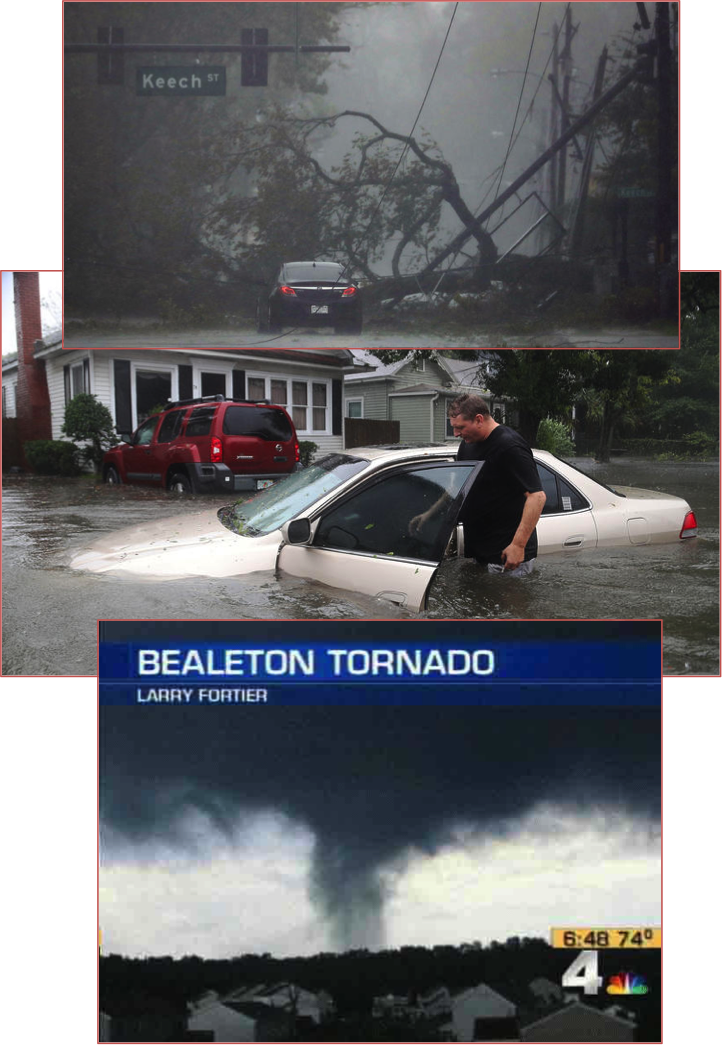
\includegraphics[width=0.8\textwidth]{storm_hazards.png}
     \end{center}
     \vspace{-0.25cm}
     \scriptsize{Image sources: Los Angeles Times, NBC}
\end{column}
\end{columns}

\end{frame}

\section{Assessing exposure}\label{assessing-exposure-3}

\begin{frame}{Distance from storm}

\large Tropical storm ``Best Track'' data \vspace{-0.7cm}

\begin{columns}
\begin{column}{0.7\textwidth}

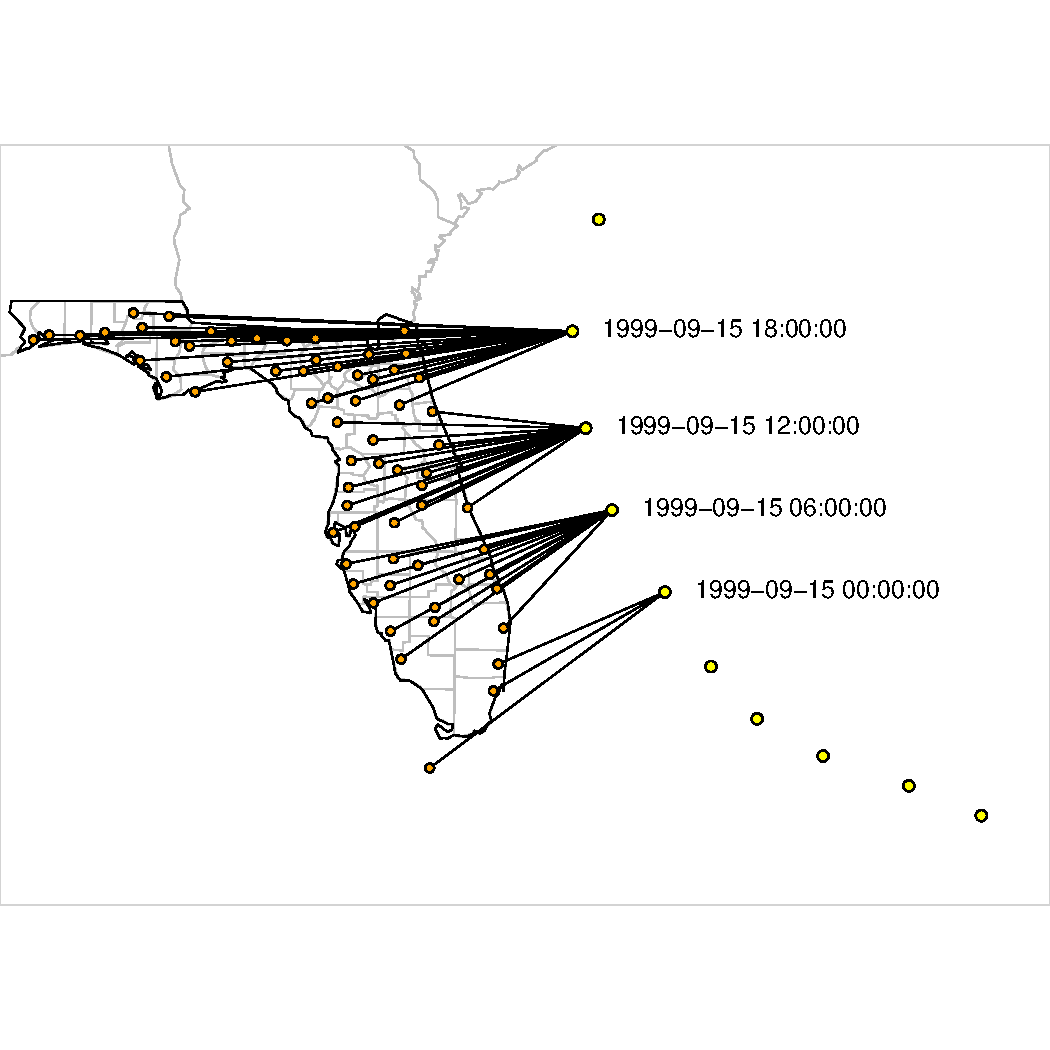
\includegraphics[width=\textwidth]{finding_closest_point} 
\end{column}
\begin{column}{0.3\textwidth}
\small
\begin{block}{Distance metric}
We matched storm tracks to county population mean centers to determine the closest approach and date of closest approach of each storm to each county.
\end{block}
\end{column}
\end{columns}

\end{frame}

\begin{frame}{Wind exposure}

\begin{columns}
\begin{column}{0.7\textwidth}

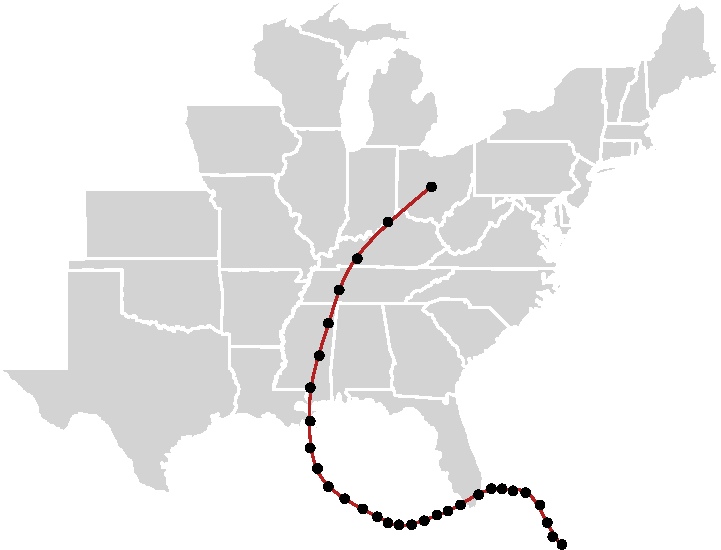
\includegraphics[width=\textwidth]{anderson_jan18_files/figure-beamer/unnamed-chunk-4-1} 
\end{column}
\begin{column}{0.3\textwidth}
\small
\begin{block}{Wind metric}
We modeled county winds with a wind model based on a Willoughby et al. paper. This model inputs storm location and maximum wind from best tracks data. 
\end{block}
\end{column}
\end{columns}

\end{frame}

\begin{frame}{Wind exposure}

\begin{block}{Details of wind model}
We have created an R package that implements this wind model. Full details on on the model implementation are available through one of the package vignettes at \url{https://cran.r-project.org/web/packages/stormwindmodel/vignettes/Details.html}. 
\end{block}

\end{frame}

\begin{frame}{Wind exposure}

\begin{center}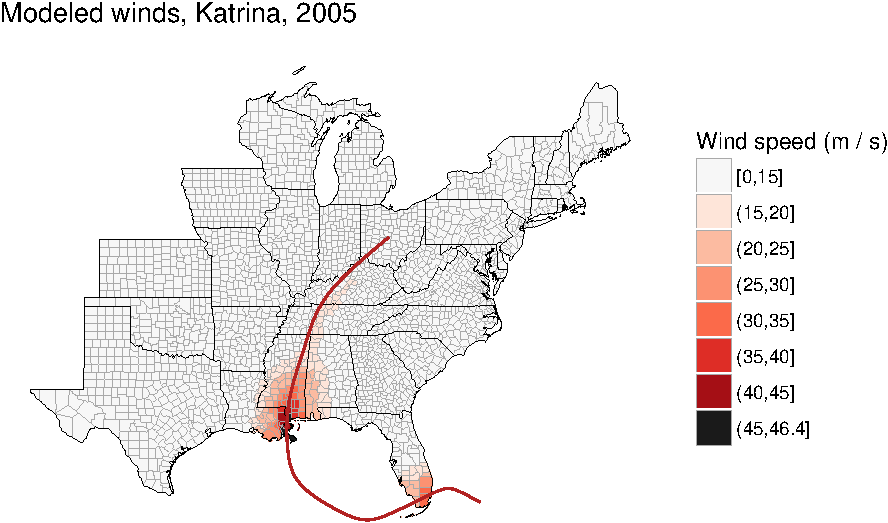
\includegraphics[width=\textwidth]{anderson_jan18_files/figure-beamer/unnamed-chunk-5-1} \end{center}

\end{frame}

\begin{frame}{Wind exposure}

\begin{block}{Assessment}
To assess results of the storm wind model, we compared modeled results with wind radii from the Extended Best Tracks for each storm. 
\end{block}

\vspace{-0.5cm}

\begin{center}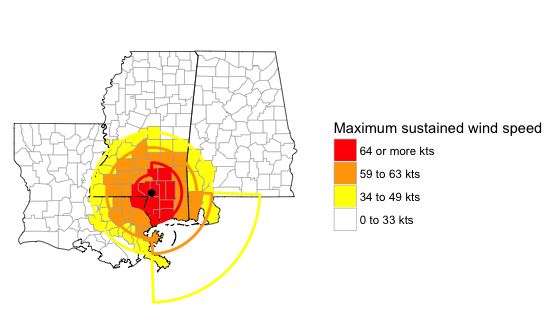
\includegraphics[width=0.75\textwidth]{ext_tracks_2} \end{center}

\end{frame}

\begin{frame}{Wind exposure}

\begin{center}
Comparison of modeled wind versus wind radii, Katrina, 2005
\end{center}

\vspace{-1cm}

\begin{flushleft}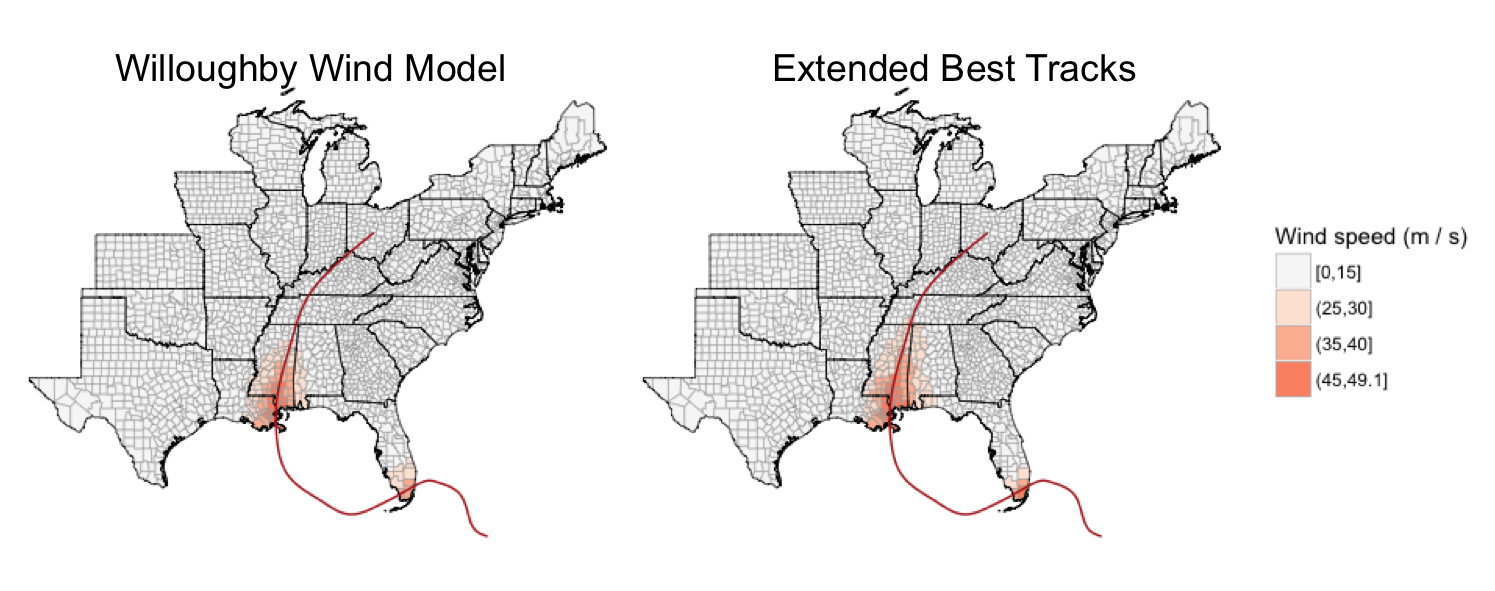
\includegraphics[width=1.08\textwidth]{wind_model_eval_katrina_2005} \end{flushleft}

\end{frame}

\begin{frame}{Wind exposure}

\begin{center}
Comparison of modeled wind versus wind radii, Ike, 2008
\end{center}

\vspace{-1cm}

\begin{flushleft}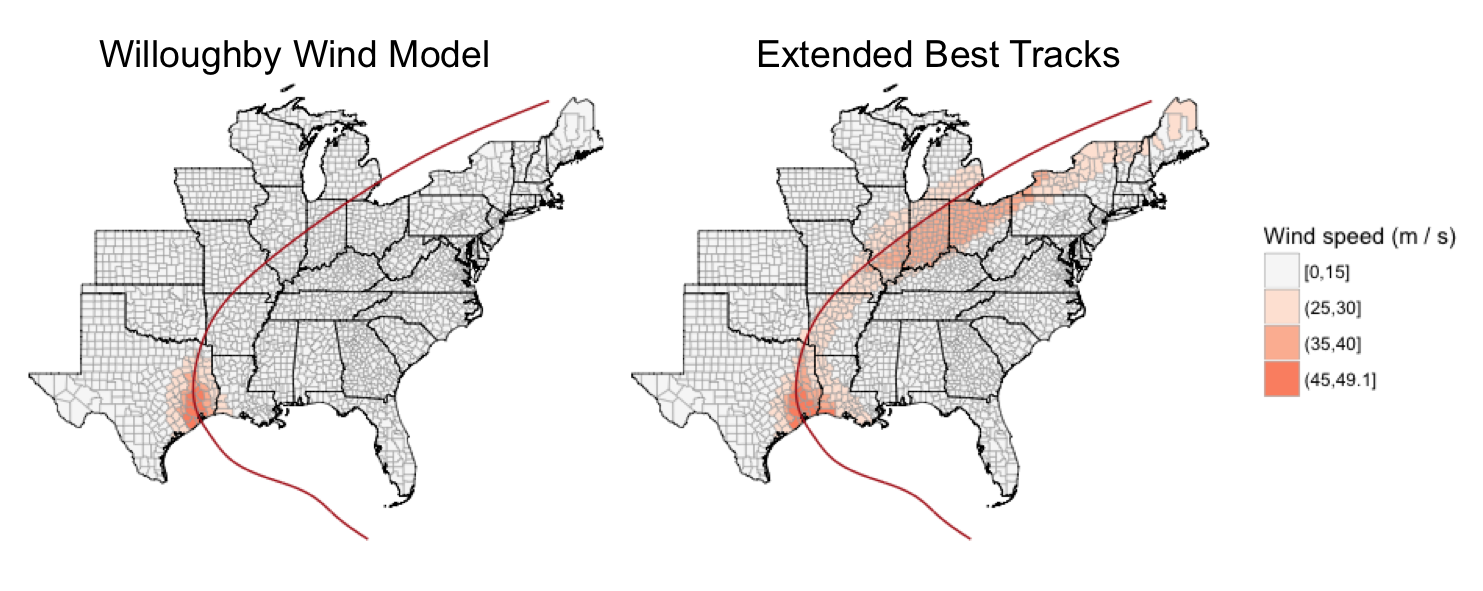
\includegraphics[width=1.05\textwidth]{wind_model_eval_ike_2008} \end{flushleft}

\end{frame}

\begin{frame}{Rain exposure}

\begin{columns}
\begin{column}{0.7\textwidth}  
    \vspace{-0.25cm}
    \begin{center}
    Rain during Tropical Storm Lee
    \end{center}
    \begin{center}
     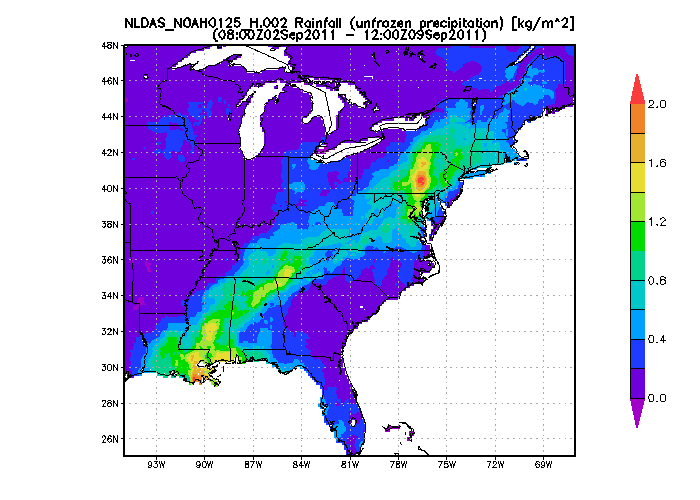
\includegraphics[width=\textwidth]{nldas2_ts_lee.png}
     \end{center}
     \begin{center}
         \vspace{-0.4cm}
     \scriptsize{Image source: Goddard Earth Sciences DISC}
     \end{center}
\end{column}
\begin{column}{0.3\textwidth}
\footnotesize
\begin{block}{Rain metric}
We used NLDAS-2 precipitation data to assess county rainfall. We summed rain from two days before to one day after the storm. We include a distance threshold for the rain metric.
\end{block}
\end{column}
\end{columns}

\end{frame}

\begin{frame}{Rain exposure}

\begin{center}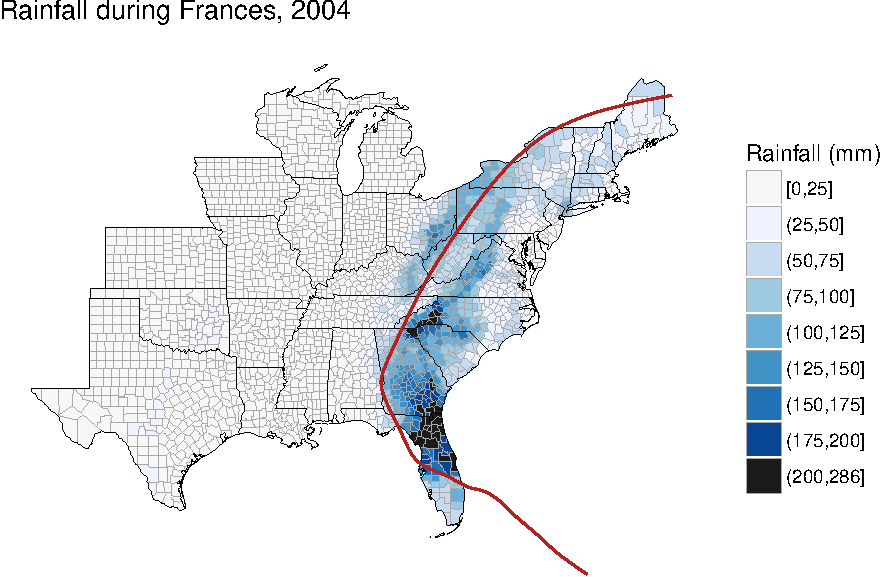
\includegraphics[width=0.9\textwidth]{anderson_jan18_files/figure-beamer/frances_rain_example-1} \end{center}

\end{frame}

\begin{frame}{Rain exposure}

\small

\begin{block}{Assessment}
To assess this rain metric, we compared it to rainfall measured at weather stations. X-axis: Rainfall summed for days near storm; y-axis: average of summed rain at each monitor for the same days.
\end{block}

\begin{flushleft}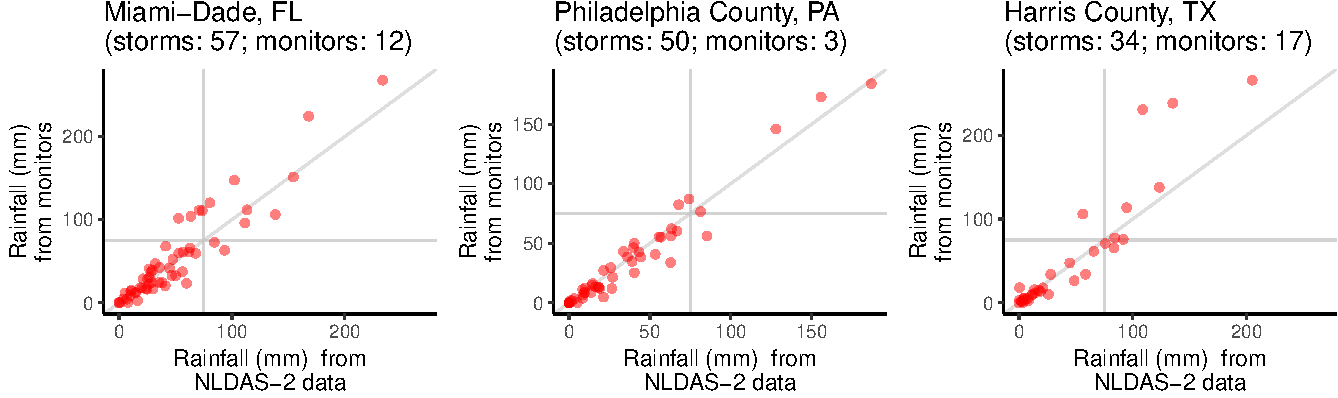
\includegraphics[width=1.05\textwidth]{anderson_jan18_files/figure-beamer/compare_rain_ex_counties-1} \end{flushleft}

\end{frame}

\begin{frame}{Rain exposure}

\begin{center}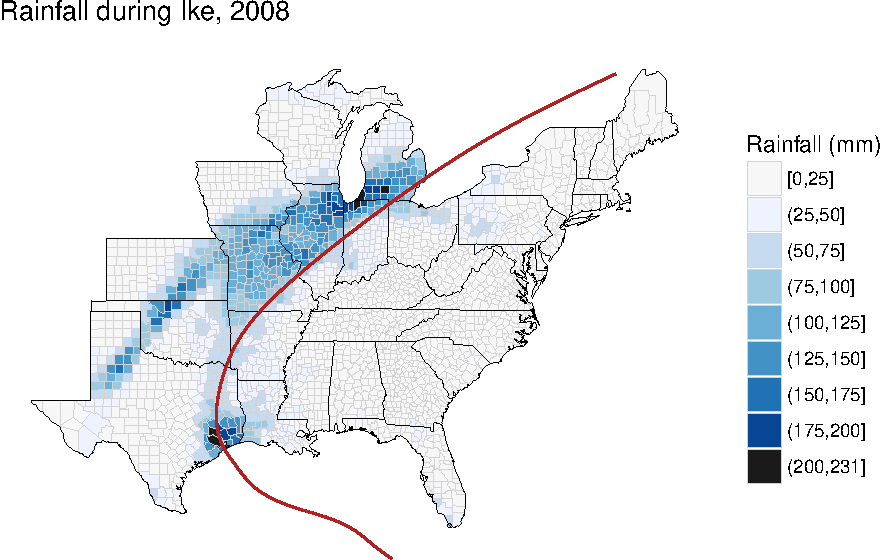
\includegraphics[width=0.9\textwidth]{anderson_jan18_files/figure-beamer/ike_rain_example-1} \end{center}

\end{frame}

\begin{frame}{Rain exposure}

\begin{center}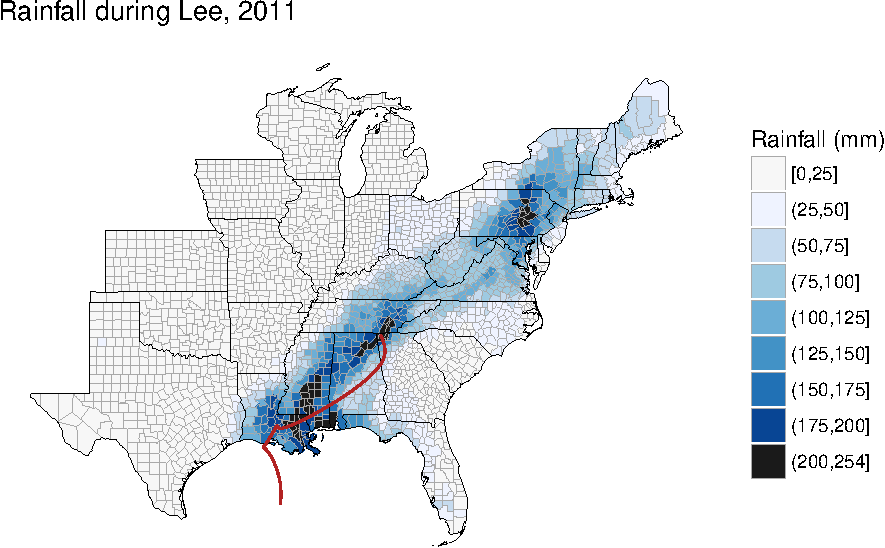
\includegraphics[width=0.9\textwidth]{anderson_jan18_files/figure-beamer/lee_rain_example-1} \end{center}

\end{frame}

\begin{frame}{Flood and tornado events}

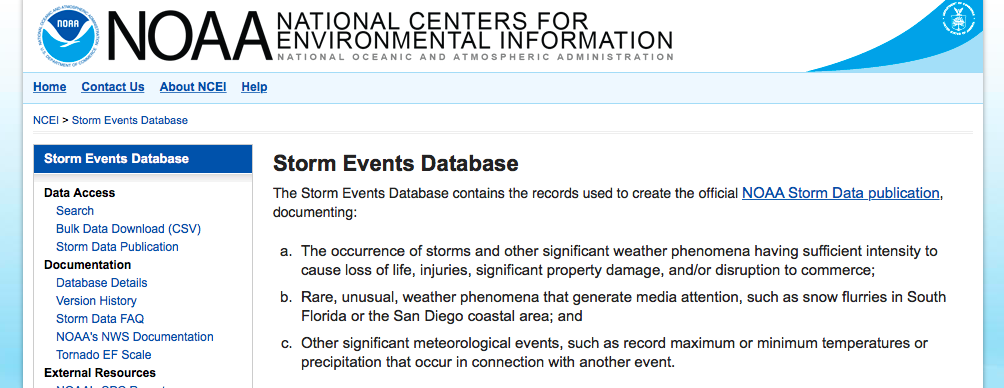
\includegraphics[width=\textwidth]{noaastormevents}

Website: \url{https://www.ncdc.noaa.gov/stormevents/}

\end{frame}

\begin{frame}{Flood and tornado events}

\begin{center}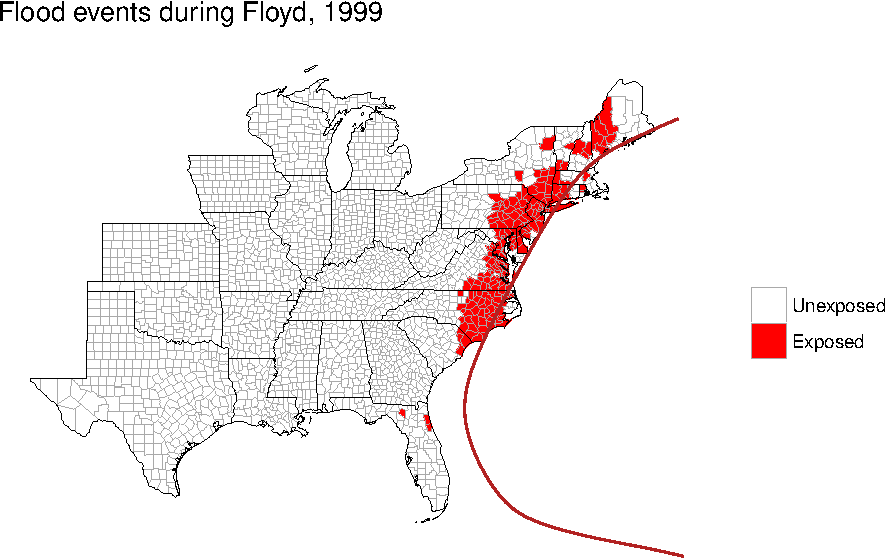
\includegraphics[width=0.9\textwidth]{anderson_jan18_files/figure-beamer/floyd_flood_example-1} \end{center}

\end{frame}

\begin{frame}{Flood and tornado events}

\begin{center}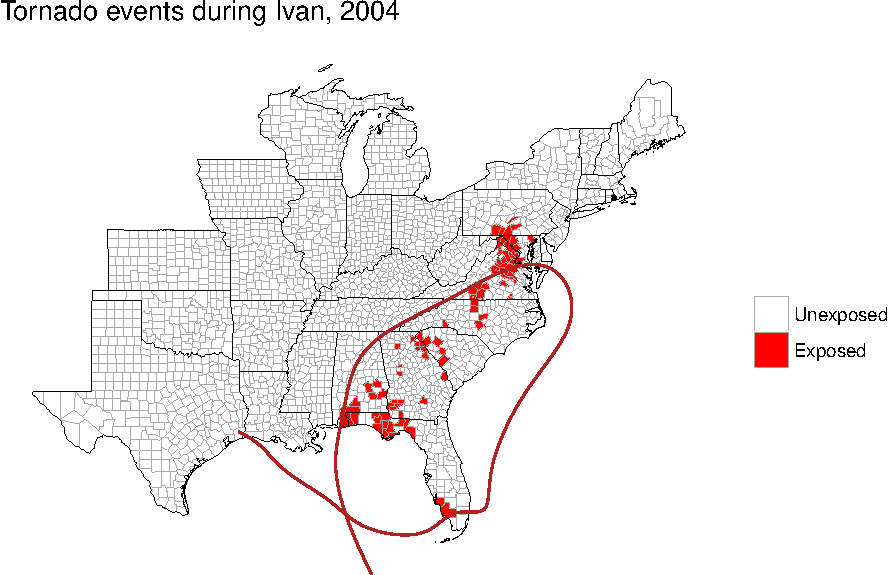
\includegraphics[width=0.9\textwidth]{anderson_jan18_files/figure-beamer/ivan_tornado_example-1} \end{center}

\end{frame}

\section{Agreement between exposure
metrics}\label{agreement-between-exposure-metrics}

\begin{frame}{Storm exposure}

\footnotesize

\begin{longtable}[]{@{}ll@{}}
\toprule
\begin{minipage}[b]{0.24\columnwidth}\raggedright\strut
Exposure metric\strut
\end{minipage} & \begin{minipage}[b]{0.68\columnwidth}\raggedright\strut
Criterial for exposure\strut
\end{minipage}\tabularnewline
\midrule
\endhead
\begin{minipage}[t]{0.24\columnwidth}\raggedright\strut
Distance\strut
\end{minipage} & \begin{minipage}[t]{0.68\columnwidth}\raggedright\strut
County population mean center within 100 km of storm track\strut
\end{minipage}\tabularnewline
\begin{minipage}[t]{0.24\columnwidth}\raggedright\strut
Rain\strut
\end{minipage} & \begin{minipage}[t]{0.68\columnwidth}\raggedright\strut
County received 75 mm or more rain over the period from two days before
to one day after the storm's closest approach and the storm passed
within 500 km of the county\strut
\end{minipage}\tabularnewline
\begin{minipage}[t]{0.24\columnwidth}\raggedright\strut
Wind\strut
\end{minipage} & \begin{minipage}[t]{0.68\columnwidth}\raggedright\strut
Modeled wind speed at county's population mean center met or exceeded 15
m / s during the storm\strut
\end{minipage}\tabularnewline
\begin{minipage}[t]{0.24\columnwidth}\raggedright\strut
Flood\strut
\end{minipage} & \begin{minipage}[t]{0.68\columnwidth}\raggedright\strut
Flood event listed with a start date within two days of the storm's
closest approach and county within 500 km of storm track\strut
\end{minipage}\tabularnewline
\begin{minipage}[t]{0.24\columnwidth}\raggedright\strut
Tornado\strut
\end{minipage} & \begin{minipage}[t]{0.68\columnwidth}\raggedright\strut
Tornado event listed with a start date within two days of the storm's
closest approach and county within 500 km of storm track\strut
\end{minipage}\tabularnewline
\bottomrule
\end{longtable}

\end{frame}

\begin{frame}{Storm exposure}

\begin{longtable}[]{@{}lcc@{}}
\toprule
\begin{minipage}[b]{0.23\columnwidth}\raggedright\strut
Exposure metric\strut
\end{minipage} & \begin{minipage}[b]{0.34\columnwidth}\centering\strut
Median number of exposed counties (IQR)\strut
\end{minipage} & \begin{minipage}[b]{0.34\columnwidth}\centering\strut
Storm with most counties exposed\strut
\end{minipage}\tabularnewline
\midrule
\endhead
\begin{minipage}[t]{0.23\columnwidth}\raggedright\strut
Distance\strut
\end{minipage} & \begin{minipage}[t]{0.34\columnwidth}\centering\strut
62 (12, 156)\strut
\end{minipage} & \begin{minipage}[t]{0.34\columnwidth}\centering\strut
Beryl, 1994 (330)\strut
\end{minipage}\tabularnewline
\begin{minipage}[t]{0.23\columnwidth}\raggedright\strut
Rain\strut
\end{minipage} & \begin{minipage}[t]{0.34\columnwidth}\centering\strut
32 (4, 133)\strut
\end{minipage} & \begin{minipage}[t]{0.34\columnwidth}\centering\strut
Frances, 2004 (464)\strut
\end{minipage}\tabularnewline
\begin{minipage}[t]{0.23\columnwidth}\raggedright\strut
Wind\strut
\end{minipage} & \begin{minipage}[t]{0.34\columnwidth}\centering\strut
26 (3, 65)\strut
\end{minipage} & \begin{minipage}[t]{0.34\columnwidth}\centering\strut
Ike, 2008 (355)\strut
\end{minipage}\tabularnewline
\begin{minipage}[t]{0.23\columnwidth}\raggedright\strut
Flood\strut
\end{minipage} & \begin{minipage}[t]{0.34\columnwidth}\centering\strut
9 (0, 39)\strut
\end{minipage} & \begin{minipage}[t]{0.34\columnwidth}\centering\strut
Ivan, 2004 (317)\strut
\end{minipage}\tabularnewline
\begin{minipage}[t]{0.23\columnwidth}\raggedright\strut
Tornado\strut
\end{minipage} & \begin{minipage}[t]{0.34\columnwidth}\centering\strut
1 (0, 9)\strut
\end{minipage} & \begin{minipage}[t]{0.34\columnwidth}\centering\strut
Ivan, 2004 (91)\strut
\end{minipage}\tabularnewline
\bottomrule
\end{longtable}

\footnotesize{\textsuperscript{*}Note: Flood and Tornado events only include storms in 1996--2011. All other event listings cover storms in 1988--2011.}

\end{frame}

\begin{frame}{Storm-specific severity}

\begin{block}{Assessing agreement in storm severity across metrics}
\begin{itemize}
\item For this assessment, we measured \textbf{storm-specific severity} as the number of counties classified as exposed by a given metric for a given storm
\item We measured this storm-specific severity for every storm and every metric (1988--2011 for distance, rain, wind; 1996--2011 for flood and tornado)
\item We measured the rank correlation (Kendall's $\tau$) between storm severity for each pair of exposure metrics 
\end{itemize}
\end{block}

\end{frame}

\begin{frame}{Storm-specific severity}

\begin{center}
\large Agreement in storm severity for distance, wind, and rain metrics
\end{center}

\begin{center}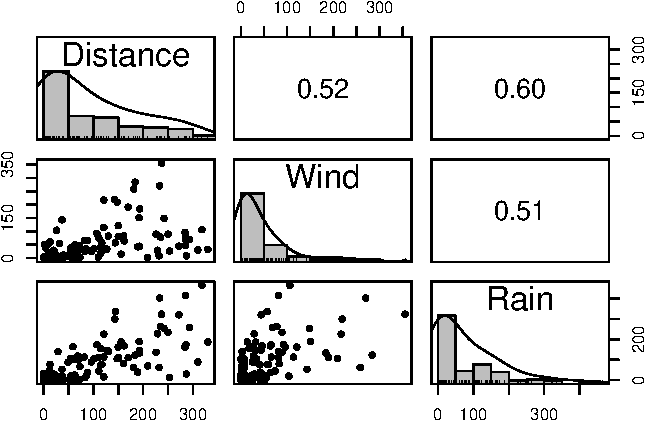
\includegraphics[width=0.7\textwidth]{anderson_jan18_files/figure-beamer/unnamed-chunk-15-1} \end{center}

\end{frame}

\begin{frame}{Storm-specific severity}

\begin{center}
\large Agreement in storm severity for exposure metrics
\end{center}

\begin{longtable}[]{@{}cccccc@{}}
\toprule
\begin{minipage}[b]{0.17\columnwidth}\centering\strut
~\strut
\end{minipage} & \begin{minipage}[b]{0.13\columnwidth}\centering\strut
Distance\strut
\end{minipage} & \begin{minipage}[b]{0.08\columnwidth}\centering\strut
Rain\strut
\end{minipage} & \begin{minipage}[b]{0.08\columnwidth}\centering\strut
Wind\strut
\end{minipage} & \begin{minipage}[b]{0.09\columnwidth}\centering\strut
Flood\strut
\end{minipage} & \begin{minipage}[b]{0.10\columnwidth}\centering\strut
Tornado\strut
\end{minipage}\tabularnewline
\midrule
\endhead
\begin{minipage}[t]{0.17\columnwidth}\centering\strut
\textbf{Distance}\strut
\end{minipage} & \begin{minipage}[t]{0.13\columnwidth}\centering\strut
-\strut
\end{minipage} & \begin{minipage}[t]{0.08\columnwidth}\centering\strut
-\strut
\end{minipage} & \begin{minipage}[t]{0.08\columnwidth}\centering\strut
-\strut
\end{minipage} & \begin{minipage}[t]{0.09\columnwidth}\centering\strut
-\strut
\end{minipage} & \begin{minipage}[t]{0.10\columnwidth}\centering\strut
-\strut
\end{minipage}\tabularnewline
\begin{minipage}[t]{0.17\columnwidth}\centering\strut
\textbf{Rain}\strut
\end{minipage} & \begin{minipage}[t]{0.13\columnwidth}\centering\strut
0.60\strut
\end{minipage} & \begin{minipage}[t]{0.08\columnwidth}\centering\strut
-\strut
\end{minipage} & \begin{minipage}[t]{0.08\columnwidth}\centering\strut
-\strut
\end{minipage} & \begin{minipage}[t]{0.09\columnwidth}\centering\strut
-\strut
\end{minipage} & \begin{minipage}[t]{0.10\columnwidth}\centering\strut
-\strut
\end{minipage}\tabularnewline
\begin{minipage}[t]{0.17\columnwidth}\centering\strut
\textbf{Wind}\strut
\end{minipage} & \begin{minipage}[t]{0.13\columnwidth}\centering\strut
0.52\strut
\end{minipage} & \begin{minipage}[t]{0.08\columnwidth}\centering\strut
0.51\strut
\end{minipage} & \begin{minipage}[t]{0.08\columnwidth}\centering\strut
-\strut
\end{minipage} & \begin{minipage}[t]{0.09\columnwidth}\centering\strut
-\strut
\end{minipage} & \begin{minipage}[t]{0.10\columnwidth}\centering\strut
-\strut
\end{minipage}\tabularnewline
\begin{minipage}[t]{0.17\columnwidth}\centering\strut
\textbf{Flood}\strut
\end{minipage} & \begin{minipage}[t]{0.13\columnwidth}\centering\strut
0.35\strut
\end{minipage} & \begin{minipage}[t]{0.08\columnwidth}\centering\strut
0.43\strut
\end{minipage} & \begin{minipage}[t]{0.08\columnwidth}\centering\strut
0.32\strut
\end{minipage} & \begin{minipage}[t]{0.09\columnwidth}\centering\strut
-\strut
\end{minipage} & \begin{minipage}[t]{0.10\columnwidth}\centering\strut
-\strut
\end{minipage}\tabularnewline
\begin{minipage}[t]{0.17\columnwidth}\centering\strut
\textbf{Tornado}\strut
\end{minipage} & \begin{minipage}[t]{0.13\columnwidth}\centering\strut
0.32\strut
\end{minipage} & \begin{minipage}[t]{0.08\columnwidth}\centering\strut
0.38\strut
\end{minipage} & \begin{minipage}[t]{0.08\columnwidth}\centering\strut
0.34\strut
\end{minipage} & \begin{minipage}[t]{0.09\columnwidth}\centering\strut
0.62\strut
\end{minipage} & \begin{minipage}[t]{0.10\columnwidth}\centering\strut
-\strut
\end{minipage}\tabularnewline
\bottomrule
\end{longtable}

\footnotesize The table gives Kendall's \(\tau\) for each pair of
exposure metrics. All comparisons that include flood or tornado metrics
are limited to storms since 1996.

\end{frame}

\begin{frame}{County-specific classification}

\begin{block}{Assessing agreement in county classifications}
For each storm and each pair of metrics, we measured the probability a county was classified as exposed by one of the metrics conditional on it being classified as exposed by the other metric:

\begin{equation}
Pr(Exposure_{Y} = 1 | Exposure_{X} = 1)
\end{equation}

\end{block}

\end{frame}

\begin{frame}{County-specific classification-- Floyd, 1999}

\begin{columns}
\begin{column}{0.6\textwidth}

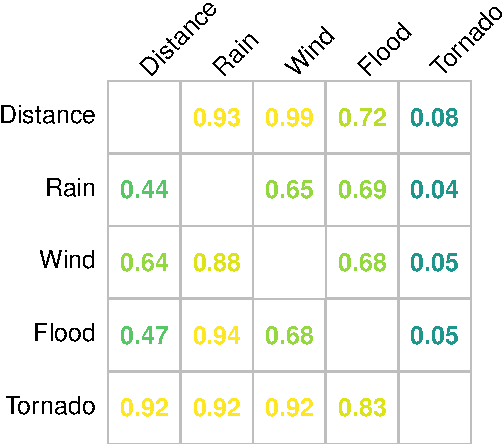
\includegraphics[width=\textwidth]{anderson_jan18_files/figure-beamer/unnamed-chunk-19-1} 
\end{column}
\begin{column}{0.4\textwidth}
\small
\begin{block}{County agreement}
Above the diagonal shows the probability that, given the county was exposed based on the metric for that row, it was also exposed based on the metric for that column. Below the diagonal shows the probability that, given the county was exposed based on the metric for that column, it was also exposed based on the metric for that row.
\end{block}
\end{column}
\end{columns}

\end{frame}

\begin{frame}{County-specific classification-- All storms}

\begin{columns}
\begin{column}{0.6\textwidth}

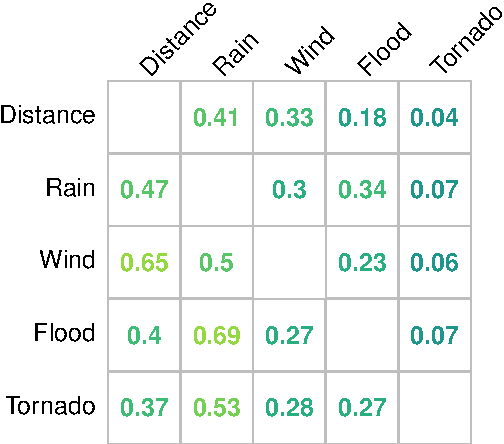
\includegraphics[width=\textwidth]{anderson_jan18_files/figure-beamer/unnamed-chunk-20-1} 
\end{column}
\begin{column}{0.4\textwidth}
\small
\begin{block}{County agreement}
Above the diagonal shows the probability that, given the county was exposed based on the metric for that row, it was also exposed based on the metric for that column. Below the diagonal shows the probability that, given the county was exposed based on the metric for that column, it was also exposed based on the metric for that row.
\end{block}
\end{column}
\end{columns}

\end{frame}

\section{Software}\label{software}

\begin{frame}[fragile]{Project software}

\footnotesize

\begin{block}{`hurricaneexposure`}
Create county-level exposure time series for tropical storms in U.S. counties. Exposure can be determined based on several hazards (e.g., distance, wind, rain), with user-specified thresholds. 
\url{https://github.com/geanders/hurricaneexposure}
\end{block}

\begin{Shaded}
\begin{Highlighting}[]
\KeywordTok{county_rain}\NormalTok{(}\DataTypeTok{counties =} \KeywordTok{c}\NormalTok{(}\StringTok{"22071"}\NormalTok{, }\StringTok{"51700"}\NormalTok{), }\DataTypeTok{rain_limit =} \DecValTok{100}\NormalTok{, }
            \DataTypeTok{start_year =} \DecValTok{1995}\NormalTok{, }\DataTypeTok{end_year =} \DecValTok{2005}\NormalTok{, }\DataTypeTok{dist_limit =} \DecValTok{100}\NormalTok{,}
            \DataTypeTok{days_included =} \KeywordTok{c}\NormalTok{(-}\DecValTok{1}\NormalTok{, }\DecValTok{0}\NormalTok{, }\DecValTok{1}\NormalTok{))}
\end{Highlighting}
\end{Shaded}

\begin{verbatim}
## # A tibble: 5 x 5
##       storm_id  fips closest_date storm_dist tot_precip
##          <chr> <chr>        <chr>      <dbl>      <dbl>
## 1    Bill-2003 22071   2003-06-30   38.78412      141.1
## 2 Charley-2004 51700   2004-08-14   43.01152      136.2
## 3   Cindy-2005 22071   2005-07-06   32.21758      113.2
## 4   Floyd-1999 51700   1999-09-16   46.50729      207.5
## 5 Isidore-2002 22071   2002-09-26    6.37844      249.0
\end{verbatim}

\end{frame}

\begin{frame}{Project software}

\vspace{-0.2cm} \large

\begin{center}
Web application interface to `hurricaneexposure`
\end{center}

\vspace{-0.3cm}

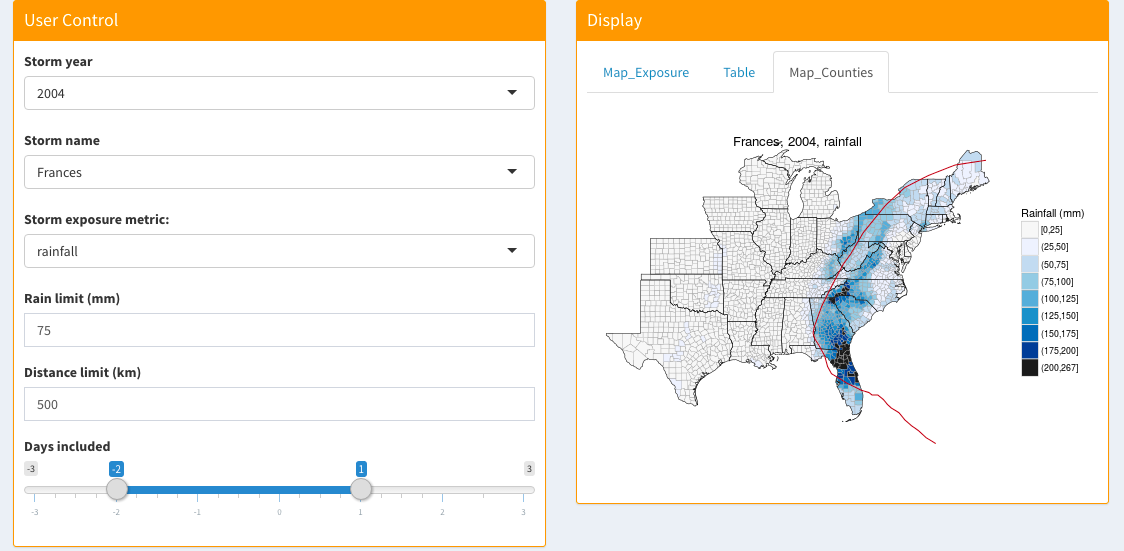
\includegraphics[width=\textwidth]{hurricane_exposure_website}

\end{frame}

\begin{frame}{Project software}

\begin{columns}
\begin{column}{0.3\textwidth}
\footnotesize
\begin{block}{`stormwindmodel`}
Model storm winds from Best Tracks data at U.S. locations. Includes modeling sustained and gust winds, as well as duration of sustained and gust winds above a specified threshold. On CRAN.
\end{block}
\end{column}
\begin{column}{0.7\textwidth}

\begin{center}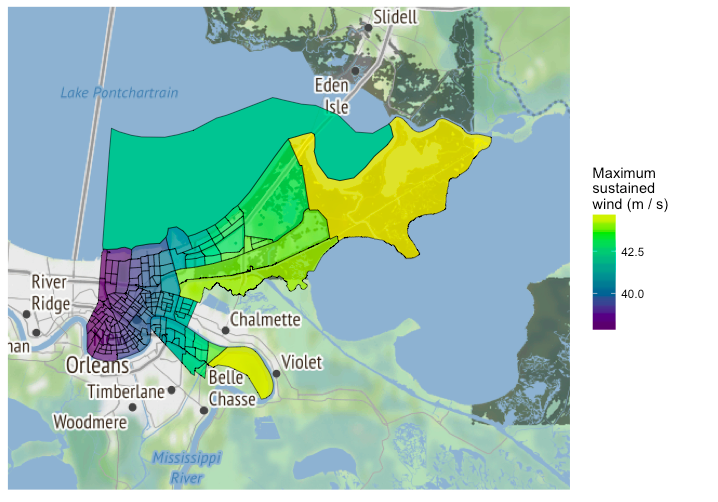
\includegraphics[width=\textwidth]{census_track_modeled_winds} \end{center}
\end{column}
\end{columns}

\end{frame}

\begin{frame}{Project software}

\footnotesize

\begin{block}{`noaastormevents`}
Download and explore listings from the NOAA Storm Events database. Includes the ability to pull events based on a tropical storm, using events listed close in time and distance to the storm's tracks. 
\url{https://github.com/zailchen/noaastormevents}
\end{block}

\footnotesize

\begin{block}{`countytimezones`}
Convert time-stamps from UTC to local time zones for U.S. counties based on county FIPs. Facilitates merging weather observations with locally measured data, including health outcomes. On CRAN.
\end{block}

\footnotesize

\begin{block}{`countyweather`}
Download weather monitor data through NOAA API by U.S. county. Includes functions to map available monitors for each county. On CRAN.
\end{block}

\end{frame}

\begin{frame}{Future work}

\begin{block}{Future work}
\begin{itemize}
\item Epidemiological study of mortality risk and tropical storm hazards
\item Exploring alternative measures of flood and tornado exposure
\item Improving wind model for extra-tropical storms
\item Incorporating metrics of infrastructure damage
\end{itemize}
\end{block}

\end{frame}

\section{R tools for open science}\label{r-tools-for-open-science}

\begin{frame}{Open data / reproducible research}

\begin{center}
\includegraphics[width=0.8\textwidth]{open_data_headlines} \end{center}

\end{frame}

\begin{frame}{Software as a research product}


\includegraphics[width=\textwidth]{coursera_screenshot}

Courses: \url{https://www.coursera.org/specializations/r} Course book:
\url{https://bookdown.org/rdpeng/RProgDA/}

\end{frame}

\begin{frame}{R package repositories}

\begin{block}{Sharing R packages}
R packages can be shared with others through: 
\begin{itemize}
  \item By sharing a \texttt{.tar.gz} file
  \item Through the Comprehensive R Archive Network (CRAN)
  \item Through GitHub (packages can be installed from GitHub with the \texttt{install\_github} function from the \texttt{devtools} package)
  \item Through a \texttt{drat} repository, hosted locally or through GitHub pages
\end{itemize}
\end{block}

\end{frame}

\begin{frame}{Software vignettes}

\begin{block}{Documenting R Software}
R packages can include \textbf{vignettes}, which provide tutorials or documentation for users. These vignettes can be written in RMarkdown, which allows a mix of executable R code and text, figures, tables, etc.
\end{block}

\begin{block}{Example vignettes}
The \texttt{stormwindmodel} package has two vignettes: 
\begin{itemize}
  \item "Overview" vignette: \url{https://cran.r-project.org/web/packages/stormwindmodel/vignettes/Overview.html}
  \item "Details" vignette: \url{https://cran.r-project.org/web/packages/stormwindmodel/vignettes/Details.html}
\end{itemize}
\end{block}

\end{frame}

\begin{frame}{Shiny web applications}

\begin{block}{Shiny web applications}
Web applications that run R code can be created using Shiny. You can use these to "wrap" an R package and make it accessible to non-R users. Shiny web apps can:
\begin{itemize}
  \item Be freely hosted through \url{https://www.shinyapps.io}
  \item Allow users to upload and download data and create figures
  \item Be extensively customized
\end{itemize}
\end{block}

\begin{block}{Help with Shiny}
\begin{itemize}
  \item Lots of tutorials are available through RStudio: \url{http://shiny.rstudio.com/}
  \item The Shiny Gallery provides simple to advanced examples, with code: \url{https://shiny.rstudio.com/gallery/}
\end{itemize}
\end{block}

\end{frame}

\begin{frame}{Peer-review options}

\begin{block}{Peer-review for R software}
R packages do not undergo peer review for CRAN and most other repositories. However, there are a few avenues for partial or full peer review of packages: \begin{itemize}
  \item \textit{ROpenSci}: Includes the option for community-contributed packages. These undergo peer review through GitHub. The full source code is reviewed and comments must be addressed before the package is added to the ROpenSci repository
  \item \textit{The Journal of Open Source Software}: Very short articles, peer review of code
  \item \textit{The R Journal}, \textit{Journal of Statistical Software}: Peer-review of articles, but may include some suggestsion for software 
\end{itemize}
\end{block}

\end{frame}

\end{document}
